%%%%%%%%%%%%%%%%%%%%%%%%%%%%%%%%%%%%%%%%%%%%%%%%%%%%%%%%%%%%%%%%%%%%%%
% How to use writeLaTeX: 
%
% You edit the source code here on the left, and the preview on the
% right shows you the result within a few seconds.
%
% Bookmark this page and share the URL with your co-authors. They can
% edit at the same time!
%
% You can upload figures, bibliographies, custom classes and
% styles using the files menu.
%
% If you're new to LaTeX, the wikibook is a great place to start:
% http://en.wikibooks.org/wiki/LaTeX
%
%%%%%%%%%%%%%%%%%%%%%%%%%%%%%%%%%%%%%%%%%%%%%%%%%%%%%%%%%%%%%%%%%%%%%%
\documentclass{tufte-handout}

%\geometry{showframe}% for debugging purposes -- displays the margins

\usepackage{amsmath}

% Set up the images/graphics package
\usepackage{graphicx}
\setkeys{Gin}{width=\linewidth,totalheight=\textheight,keepaspectratio}


\usepackage{color, colortbl}

%Portuguese-specific commands
%--------------------------------------
\usepackage[portuguese, english]{babel}
\selectlanguage{portuguese}
%--------------------------------------
 
%Hyphenation rules
%--------------------------------------
\usepackage{hyphenat}
\hyphenation{mate-mática recu-perar}
%--------------------------------------


% fix pro tufte no xetex (q preciso para fontes customizadas)
% https://tex.stackexchange.com/a/202189
\usepackage{ifxetex}
\ifxetex
  \newcommand{\textls}[2][5]{%
    \begingroup\addfontfeatures{LetterSpace=#1}#2\endgroup
  }
  \renewcommand{\allcapsspacing}[1]{\textls[15]{#1}}
  \renewcommand{\smallcapsspacing}[1]{\textls[10]{#1}}
  \renewcommand{\allcaps}[1]{\textls[15]{\MakeTextUppercase{#1}}}
  \renewcommand{\smallcaps}[1]{\smallcapsspacing{\scshape\MakeTextLowercase{#1}}}
  \renewcommand{\textsc}[1]{\smallcapsspacing{\textsmallcaps{#1}}}
  \usepackage{fontspec}
\fi


\usepackage{fontspec}
\setmainfont[
    Path=./Literata/,
    BoldFont=Literata-Bold,
    ItalicFont=Literata-Italic,
    BoldItalicFont=Literata-BoldItalic,
]{Literata-Regular}

\title{Letras que ecoem a fala: tipografia modulada por prosódia}
%\title{A voz na letra: tipografia modulada pela fala}

\author{Caluã de Lacerda Pataca, Paula Dornhofer Paro Costa}
\date{24 de novembro de 2019}  % if the \date{} command is left out, the current date will be used

% The following package makes prettier tables.  We're all about the bling!
\usepackage{booktabs}

% The units package provides nice, non-stacked fractions and better spacing
% for units.
\usepackage{units}

% The fancyvrb package lets us customize the formatting of verbatim
% environments.  We use a slightly smaller font.
\usepackage{fancyvrb}
\fvset{fontsize=\normalsize}

% Small sections of multiple columns
\usepackage{multicol}

% Provides paragraphs of dummy text
\usepackage{lipsum}

% These commands are used to pretty-print LaTeX commands
\newcommand{\doccmd}[1]{\texttt{\textbackslash#1}}% command name -- adds backslash automatically
\newcommand{\docopt}[1]{\ensuremath{\langle}\textrm{\textit{#1}}\ensuremath{\rangle}}% optional command argument
\newcommand{\docarg}[1]{\textrm{\textit{#1}}}% (required) command argument
\newenvironment{docspec}{\begin{quote}\noindent}{\end{quote}}% command specification environment
\newcommand{\docenv}[1]{\textsf{#1}}% environment name
\newcommand{\docpkg}[1]{\texttt{#1}}% package name
\newcommand{\doccls}[1]{\texttt{#1}}% document class name
\newcommand{\docclsopt}[1]{\texttt{#1}}% document class option name



\makeatletter
\renewcommand{\fnum@figure}{Fig.~\thefigure}
\renewcommand{\fnum@table}{Tabela~\thetable}
\makeatother


\begin{document}

\maketitle% this prints the handout title, author, and date

\begin{abstract}
\noindent Hello World.
\end{abstract}

%\printclassoptions

\section{Objetivos e justificativas do projeto de pesquisa}\label{sec:objetivos}
%\subsection{Headings}\label{sec:headings}

Em um filme, as legendas traduzem em texto aquilo que falam as personagens. Sons codificados tipograficamente dão acesso ao \textit{que} é dito, mas essa representação ignora \textit{como} as palavras são ditas. Nosso trabalho parte da ideia de que, dado que os sentidos do \textit{que se diz} são modificados por \textit{como se diz}, um sistema de legendas poderia buscar representações visuais que permitissem a seus espectadores intuir qualidades expressivas na voz das personagens e, assim, ter uma experiência audiovisual mais rica.

Tal sistema poderia ganhar usos como um componente de aplicações de acessibilidade, em especial considerando um público com deficiências auditivas que, a princípio, é excluído de toda uma dimensão expressiva quando assiste a conteúdos audiovisuais. Além desse uso mais restrito, imaginamos que, da mesma forma que as \textit{closed captions} trazem benefícios para públicos em geral, ouvintes ou não\sidenote[][-1\baselineskip]{Filmes legendados produzem melhoras na compreensão, atenção e memória em diversos públicos: crianças, adultos ou idosos; leitores experientes ou em fase de aprendizado; falantes ou não da língua em questão; ouvintes ou com deficiências auditivas; etc. \citep{fiske_video_2015}}, uma legenda expressiva poderia ganhar usos além das tecnologias assistivas.

Dentro deste projeto de mestrado, o escopo do trabalho circula em torno da criação de um protótipo que permita interpretar computacionalmente falas expressivas para então codificá-las, também computacionalmente, enquanto representações tipográficas. Além de desenvolvê-lo, buscaremos avaliar diferentes aspectos desse modelo ``prosódico-tipográfico'', visando tanto medir seus efeitos quanto melhor entendê-los.

\section{Revisão bibliográfica resumida}\label{sec:revisao_bibliografica}

Nosso estudo é fundado na noção de que a prosódia da fala compreende uma dimensão emocional. Trata-se de uma constatação simples: o mesmo trato vocal que molda a fala é parte de um corpo que, sob efeito de diferentes estados emocionais, se tensiona e relaxa de diversas maneiras. A emoção não é, claro, a única dimensão que modula os parâmetros acústicos da prosódia.\sidenote[][-3\baselineskip]{Ainda que não tenhamos tratado a questão nos dois primeiros experimentos já realizados, o fato de que variações prosódicas em geral compreendem diversos aspectos além da emoção é um desafio importante em nosso trabalho.} Diferentes autores dividem as funções da prosódia de diferentes maneiras \citep{schotz2002linguistic}, mas para nossos propósitos cabe citar aqui três aspectos: o linguístico, paralinguístico e extralinguístico: 

\begin{quotation}
    Enquanto o conteúdo verbal -- efetivamente o significado das palavras -- é considerado como informação linguística, o canal extralinguístico contém informações sobre o estado base do falante, e.g. uma pessoa grande (...) terá uma voz mais grave do que a de uma criança. Alguns parâmetros extralinguísticos são também determinados pela cultura do falante. (...) O canal paralinguístico carrega informações sobre desvios passageiros da linha de base típica (extralinguística), tais como (...) a expressão de emoções. \sidenote[][-11\baselineskip]{\begin{otherlanguage}{english}
    \textit{Whereas the verbal content, the actual meaning of the words, is thought of as linguistic information, the extralinguistic channel contains information about the speaker's basic state, e.g. a big person (...) will usually have a lower voice than a child. Some extralinguistic parameters are also determined by the culture of the speaker. (...) The paralinguistic channel carries information about momentary deviations from the usual (extralinguistic) baseline, such as (...) the expression of emotions.} \end{otherlanguage} \citep{quast2001automatic}}
\end{quotation}

A presença de aspectos emocionais na prosódia com algum grau de independência de aspectos linguísticos é explorada em \citet{SILVA2016}, onde um conjunto de áudios em português natural foi avaliado por brasileiros e suecos. Ainda que entre os brasileiros tenha havido maior grau de concordância nas respostas, os suecos, para quem o componente linguístico dos áudios era indiferente, também conseguiram decodificar emoções.

Essas três dimensões prosódicas (linguística, para- e extra-) são articuladas pela produção e recepção de três parâmetros acústico-perceptuais \sidenote[][-1\baselineskip]{Como mostra \citet{livroDoPlinio}, a relação entre produção e percepção não é linear e esses parâmetros se entrelaçam: mudanças em um causam diferenças de percepção em outro.}, que modificam cada sílaba em relação às demais: intensidade (mais fraca ou forte), \textit{pitch} (mais aguda ou grave) e duração (mais lenta ou rápida).

Parte dessas variações é codificada na linguagem escrita, parte não. Com efeito, a história da escrita acompanha inúmeras mutações em convenções -- inicialmente caligráficas, eventualmente tipográficas -- que, muitas vezes, estão relacionadas à variações na representação de atributos prosódicos. 

\begin{marginfigure}
  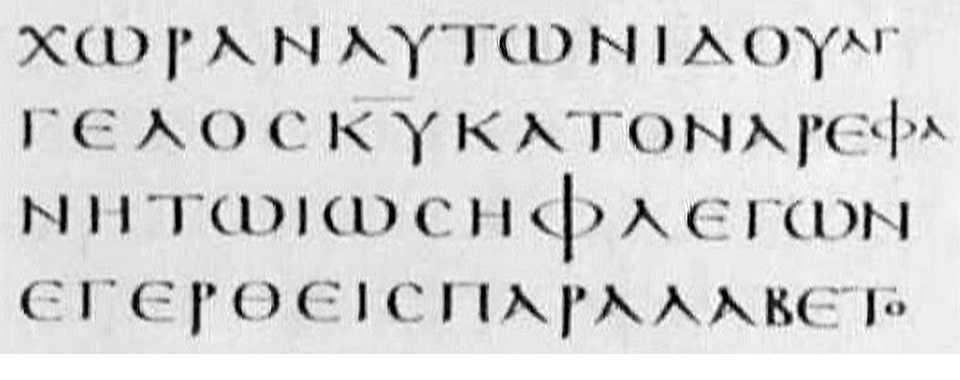
\includegraphics{imgs/codex.png}
  \caption{Trecho do \textit{Codex Vaticanus}, datado do século \textsc{iv}, exemplo de \textit{scriptio continua}. \citep{codex_vaticanus}}
  \label{cdx_vat}
\end{marginfigure}

Até que fossem introduzidos no século \textsc{vii}, não se usavam espaços ou outros sinais para separar as palavras, o texto um bloco fechado de letras -- a partir do que alguns historiadores avançam a teoria\sidenote[][\baselineskip]{Popular, mas bastante controversa. Ver \citet{McCutcheon2015}.} de que a literatura na antiguidade era predominantemente acústica \citep{kuster2016}: a leitura se fazia necessariamente em voz alta pois só ao converter em sons o ``bloco'' este se tornava compreensível. O texto então seria ``melhor percebido pelos ouvidos do que pelos olhos.'' \citep{nunlist1991}

Inovação medieval (ou não), a leitura silenciosa não é, como talvez se possa imaginar, desprovida de prosódia. Dentre as estruturas cerebrais envolvidas no processo de leitura, é surpreendente notar que, além das estruturas encarregadas do processamento semântico e ortográfico, a leitura demanda também aquelas tipicamente relacionadas à produção e processamento de sons \citep[cap.~7]{seidenberg2017}. Isso ocorre porque, mesmo quando lê silenciosamente, cabe ao leitor deduzir em sua voz interna uma representação sonora do texto, habilidade fundamentalmente relacionada à compreensão e interpretação do mesmo.

O bom funcionamento dessa ``voz'' interna é importante. Certos tipos de dislexia, por exemplo, parecem antes causados por problemas nessas estruturas fonológicas do que deficiências nas processamento de imagens, mesmo que se manifestem sob a forma de dificuldades na  leitura \citep[cap.~8]{seidenberg2017}. Ao contrário da noção vendida por certos cursos de leitura dinâmica de que uma leitura sem subvocalização traria ganhos de velocidade sem perdas na compreensão, o leitor experiente depende dessa voz interna para reduzir ambiguidades e facilitar a compreensão \citep[cap.~4]{seidenberg2017}. Finalmente, crianças em processo de alfabetização que leem de maneira monótona tendem a desenvolver problemas de compreensão \citep{bessemans2017}.

A partir da hipótese de que a falta de representação prosódica na tipografia seria um empecilho na alfabetização, a pesquisadora belga Ann Bessemans e seu grupo têm estudado um tipo de intervenção no texto que busca ajudar crianças a ler expressivamente. No estudo, a prosódia é codificada visualmente em atributos tipográficos: texto em \textit{negrito} quando lido com maior volume, \textit{espremido} quando mais rápido, \textit{esticado} quando mais lento e \textit{elevado} quando agudo. Seus resultados iniciais mostram que as crianças conseguiram entender e integrar essas dicas visuais na sua leitura, indicando o potencial da abordagem como uma representação intuitiva da expressividade da voz. \citep{bessemans2017}

\citet{wolfel2015} criaram o \textit{Design de Tipos Orientado pela Voz} (\textsc{vdtd}, sigla para \textit{Voice Driven Type Design}), uma abordagem semelhante à de Bessemans mas de base computacional. Nela, mapeiam atributos acústicos de cada fonema -- como intensidade, \textit{pitch} e velocidade -- em grafemas em uma fonte geométrica matematicamente modelada e cujos atributos podem ser manipulados. Em uma avaliação com leitores, foram encontrados indícios tanto de que as características da fala conseguiram ser impressas no texto quanto que uma abordagem nessa linha poderia ser usada para representar emoções presentes na voz. \sidenote[][-6\baselineskip]{O \textsc{vdtd} serviu como grande inspiração para nosso próprio trabalho, mas buscamos divergir no que consideramos duas falhas em sua abordagem: (1) o uso de uma tecnologia tipográfica própria é um grande empecilho para a eventual adoção da tecnologia nos já existentes ambientes de uso de tipografia digital; (2)~a avaliação foi construída principalmente com questionários onde um pequeno número de participantes fez autorrelatos de suas impressões, o que significa que os (pequenos) efeitos medidos são difíceis de generalizar.}




\break



Prosódia como representação do estado emocional do falante. Estudo do Plínio.

Discussão sobre emoção interpretada vs representação de atributos acústicos.

Discussão sobre legendas.

\section{Metodologia utilizada}\label{sec:metodologia}

\subsection{Extração e representação de prosódia}\label{sec:met_extract_represent}

\subsection{Experimento \#1: Card sorting e entrevistas com designers}\label{sec:met_exp_2}

\subsection{Experimento \#2: Associação entre emoções, \textit{features} prosódicas e eixos tipográficos}\label{sec:met_exp_2}

\subsection{Experimento \#3: }\label{sec:met_exp_2}

\section{Plano de trabalho e cronograma}\label{sec:plano_de_trabalho}

\section{Resultados e conclusões parciais}\label{sec:resultados}

\subsection{O primeiro experimento}

Os resultados do primeiro experimento talvez valham mais pelo que as entrevistas revelaram do que propriamente pelas \textit{edit-distances} medidas nas organizações dos cartões. Estas deveriam medir se os participantes conseguiram intuir na tipografia aspectos do estado emocional da voz da atriz que leu  as frases impressas nos cartões, mas o efeito capturado foi muito pequeno: a \textit{edit-distance} média no experimento é, na média, apenas 2\% menor que a que se poderia esperar caso os participantes simplesmente sorteassem as posições de cada cartão (cf. Figura~\ref{edit_dist_1}).

\begin{marginfigure}
  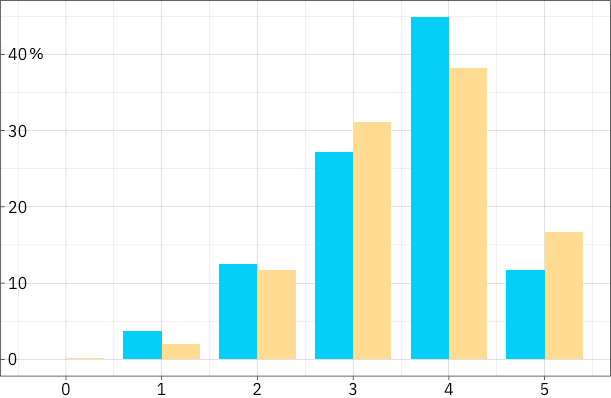
\includegraphics{imgs/edit_distance_reais.png}
  \caption{\textit{Edit-distances} das organizações coletadas (em azul) \textit{vs} uma organização ``aleatória'' (em amarelo).}
  \label{edit_dist_1}
\end{marginfigure}

Aqui, não pudemos intuir se nos dados estávamos vendo que nossa tipografia modulada pela fala era ineficaz ou se estávamos sofrendo com o mau desenho do experimento. Talvez, apostamos, seja mais o segundo caso: o modo como configuramos o \textit{card sort} pode ter conduzido a altas taxas de erro. Como \textit{todos} os cartões deveriam necessariamente ser atribuídos a uma emoção, estão embaralhados em nossos resultados coletados tanto cartões em que o participante tinha algum grau de certeza sobre a emoção quanto aqueles em que houve um ``chute.''\sidenote[][-1\baselineskip]{E, para piorar, no \textit{card sort} um cartão errado implicará necessariamente em um segundo cartão também errado.} Temos motivos para crer que esses chutes foram comuns, pois, tanto nas entrevistas quanto espontaneamente durante a atividade, muitos participantes nos relataram que a atividade era muito difícil.

A essa dificuldade da atividade em si soma-se o fato de que misturamos no experimento, e sem nenhuma forma de controle que isolassem seus efeitos, variações de três \textit{features} prosódicas com três eixos tipográficos associados a seis emoções. Dado esse cenário, não é de se espantar que com os dados coletados nos foi muito difícil responder quão bem (ou mal) nosso modelo prosódico-tipográfico representava a voz da atriz em cada uma das emoções presentes. 


\begin{marginfigure}
  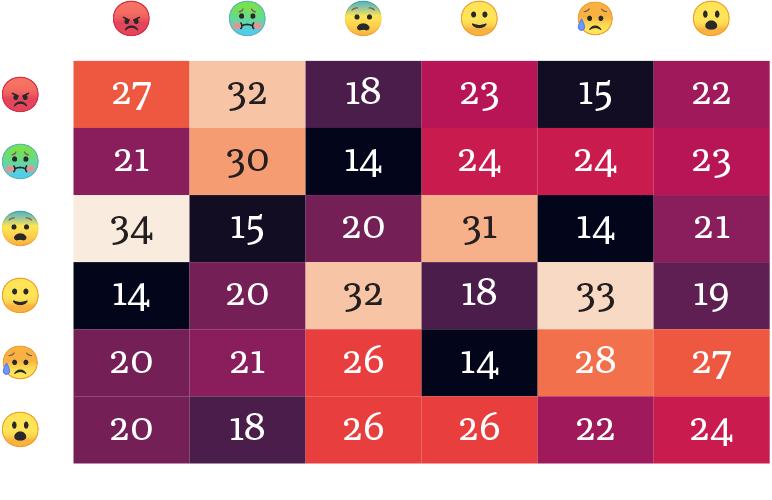
\includegraphics{imgs/confusion-emoji2.png}
  \caption{Matriz de confusão do experimento de \textit{card sort}. Emoção da atriz nas linhas, classificação dos participantes nas colunas.}
  \label{matriz_confusao}
\end{marginfigure}

Na tentativa de encontrar explicações alternativas para o baixo ganho no \textit{edit-distance}, nos perguntarmos se certos aspectos do modelo prosódico-tipográfico não estariam fazendo os participantes trocarem uma emoção por outra. Esta hipótese nos ocorreu na análise da matriz de confusão da Figura~\ref{matriz_confusao}, que parece indicar uma possível troca feita pelos participantes especificamente entre os cartões representando medo e alegria (terceira e quarta linhas e colunas). Teria o modelo invertido o sentido de alguma das features ou eixos tipográficos em relação ao que seria intuitivo? Para testar a hipótese, calculamos novamente a \textit{edit-distance}, desta vez considerando que os cartões com medo seriam de alegria e vice-versa. Como mostra a Figura~\ref{edit_dist_2}, a performance melhora (8\% de ganho em relação à distribuição aleatória). Mas o efeito continua pequeno.

\begin{marginfigure}[0.5\baselineskip]
  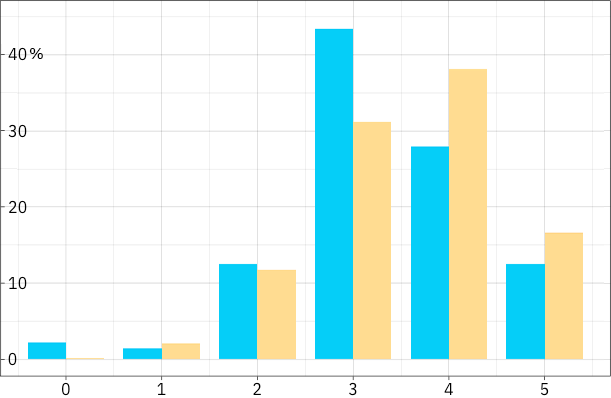
\includegraphics{imgs/edit_distance_troca.png}
  \caption{\textit{Edit-distances} das organizações coletadas, mas com troca alegria--medo (em azul) \textit{vs} uma organização ``aleatória'' (em amarelo).}
  \label{edit_dist_2}
\end{marginfigure}

O que nos disseram as entrevistas? Além do muito frequente comentário de que a avaliação era muito difícil, emergiram alguns padrões em como os participantes interpretaram as modulações tipográficas. De longe o atributo mais citado, aumento no \textit{peso} foi quase unanimemente associado a maior volume na voz, ainda que foram poucos os que perceberam que pesos leves estavam relacionados a volumes baixos na voz.

Em relação aos outros dois eixos houve grande difusão de comentários. Sobre a \textit{inclinação}, houve quem a interpretasse como velocidade, fraqueza, tristeza, ou mesmo alguns que notaram as modulações nesse eixo mas que não souberam decodificá-las. \textit{Largura} foi citada por apenas um participante, que intuiu corretamente que seu aumento e baixa estavam relacionados a oscilações de duração na pronúncia das sílabas.

Comentando sobre estratégias usadas para classificar cada cartão, emergiram dois principais grupos: no primeiro, mais frequente, o participante olhava para o cartão e buscava ``soá-lo'' mentalmente\sidenote{Ou, mais raramente, em voz baixa, como notamos em alguns casos.}, tentando interpretar em sons as modulações visuais nas letras. O segundo grupo ia no sentido oposto: tentava fazer soar a frase como que sob o efeito de cada uma das seis emoções para só então buscar nos cartões aquele cuja tipografia se aproximasse do som.

Como muitos participantes sequer perceberam as modulações de \textit{largura} e que houve grande divergência em como foram interpretadas as modulações de \textit{inclinação}, podemos supor que ambas as estratégias relatadas sofrem de um mesmo problema: se apenas os momentos mais gritados foram bem capturados, grande parte da expressividade na voz da atriz se perdeu e, não só isso, essa perda compromete de maneira desigual cada uma das emoções.\sidenote[][-2\baselineskip]{\citet{deMoraes2016} mostram como variações nas \textit{features} de \textit{f0} e duração são sensíveis à expressão de diferentes emoções na voz.}

\subsection{O segundo experimento}

Os resultados do segundo experimento, sintetizados na tabela~\ref{tab:type_perf}, são mais esclarecedores. Ao cruzar como interagem as dimensões emoção na voz, \textit{feature} prosódica e eixo tipográfico, é possível perceber que as preferências dos participantes não seguem um padrão único, variando de acordo com as diferentes possíveis combinações dessas dimensões. Pode-se vislumbrar assim que uma representação bem sucedida de qualidades expressivas da prosódia teria que ponderar os atributos dessa mesma prosódia para só então determinar quais eixos tipográficos modular.


\begin{table}
    \small
    \caption{Preferência dos participantes por cada modulação tipográfica quando usada com cada uma das emoções (considerando a média entre as duas frases testadas). \newline A preferência de 83\% para \textit{peso} quando usado para representar \textsc{rms} na frase com raiva, por exemplo, indica que ela foi escolhida em 83\% das vezes em que foi colocada contra os outros três eixos. \newline Células em verde indicam que uma dada combinação de eixo tipográfico e \textit{feature} prosódica obteve a maior preferência dentre todas as possibilidades testadas. Células em cinza indica maior preferência apenas para aquela determinada \textit{feature}. \newline Não elegemos uma preferência para tristeza pois nela a distribuição das preferências não foi estatisticamente significante.}
    \label{tab:type_perf}
    \resizebox{\textwidth}{!}{%
    \begin{tabular}{lcccc}
        \toprule
        \multicolumn{5}{c}{ \textbf{\textsc{rms} enquanto \textit{feature} representada.} }     \\
        \midrule
        emoção na voz & peso & larg. horiz. & inclinação & desloc. vert.  \\
        \midrule
        raivosa & \cellcolor[HTML]{dddddd}83\% & 34\% & 43\% & 39\% \\
        feliz & 34\% & 54\% & 47\% & \cellcolor[HTML]{dddddd}64\% \\
        neutra & 47\% & 52\% & \cellcolor[HTML]{9ef7cd}76\% & 25\% \\
        triste & 45\% & 52\% & 46\% & 58\% \\
        surpresa & \cellcolor[HTML]{9ef7cd}72\% & 38\% & 49\% & 43\% \\
        \midrule
        \multicolumn{5}{c}{ \textbf{\textit{f0} enquanto \textit{feature} representada.} }      \\
        \midrule
        emoção na voz & peso & larg. horiz. & inclinação & desloc. vert.  \\
        \midrule
        raivosa             & \cellcolor[HTML]{9ef7cd}87\% & 46\% & 45\% & 26\% \\
        feliz & 28\% & 66\% & 40\% & \cellcolor[HTML]{9ef7cd}69\% \\
        neutra & 47\% & 55\% & \cellcolor[HTML]{dddddd}63\% & 35\% \\
        triste & 21\% & 57\% & 39\% & \cellcolor[HTML]{9ef7cd}79\% \\
        surpresa & \cellcolor[HTML]{dddddd}71\% & 43\% & 41\% & 44\% \\
        \bottomrule
    \end{tabular}}
\end{table}

Essa constatação, se verdadeira, carrega uma explicação possível para pelo menos parte do insucesso na abordagem testada no primeiro experimento: ao combinar sempre da mesma maneira as três \textit{features} prosódicas com os mesmos três eixos tipográficos, tínhamos uma tipografia que coincidia com as expectativas dos participantes apenas em parte dos cartões.

Por exemplo: se, como nos mostra a tabela~\ref{tab:type_perf}, as pessoas não acham que o eixo \textit{peso} produz boas representações do \textsc{rms} em uma voz feliz, o fato de que assim o usávamos também nos cartões em que a atriz simulou felicidade pode tê-los aproximado da raiva ou da surpresa, emoções onde o \textit{peso} parece mais apropriado.

\begin{marginfigure}[15\baselineskip]
  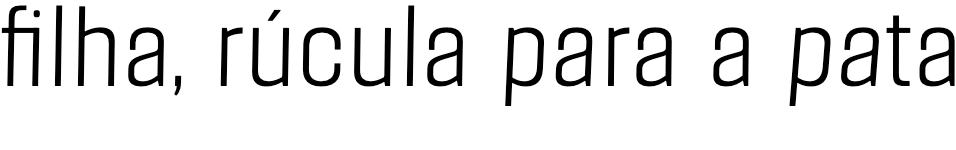
\includegraphics{imgs/slight-slant.png}
  \caption{\textit{Inclinação} como representação de \textsc{rms} na versão neutra da frase.}
  \label{slight_slant}
\end{marginfigure}

Outra conclusão interessante é que tanto \textit{largura horizontal} quando \textit{inclinação}, pouco citados nas entrevistas do primeiro experimento, tem em geral uma performance mediana, com a preferência geral tendendo à inclinação apenas quando esta é associada a uma emoção que é diferente de todas as outras: a voz neutra. De fato, como pode-se notar na figura~\ref{slight_slant}, eleita a representação mais fiel da voz neutra, as modulações tipográficas aqui são praticamente imperceptíveis. Mas esse resultado não estranha: talvez estas tenham sido as escolhas dos participantes justamente porque, em vozes que buscam ser inexpressivas, as melhores representações seriam aquelas nas quais quase não haja modulação tipográfica. Se for mesmo esse o caso, pode-se supor que uma abordagem que pondere os atributos prosódicos para só então determinar quais eixos tipográficos modular deve considerar também a possibilidade de, para determinadas vozes, \textit{não modular eixo algum}.

Uma última discussão se dá com os comentários deixados pelos participantes. Muitos desses textos discorrem sobre como foram interpretadas as modulações tipográficas. Notamos que cada eixo foi associado a diversas qualidades -- agressividade e firmeza para o \textit{peso}; uma voz melódica, quase cantada, ou divertida, ou ainda bêbada para o \textit{deslocamento vertical}; uma voz tímida para a~\textit{largura horizontal;} etc. 

Surge que, nesse compêndio de qualidades, mesmo que as respostas tenham vindo difusas, cada uma trazendo adjetivos diferentes entre si, de um modo geral os participantes parecem não estar descrevendo os atributos \textit{acústicos} da prosódia que os eixos tipográficos representavam e tampouco as seis emoções que a atriz buscou representar. Antes, as descrições falam de vozes \textit{modificadas}, como se os participantes não tenham deduzido nem nosso modelo prosódico-tipográfico nem, como esperávamos no primeiro experimento, as emoções que a atriz buscou representar, mas sim uma interpretação própria que assimila emoção \textit{e}~acústica.

Esse resultado condiz com o que discutem Boehner et al. quando apontam que ``a comunicação de afetos em um modelo interacional (...) é mais do que a mera transmissão, (...) requerindo das partes uma interpretação ativa.'' \sidenote[][-1\baselineskip]{\begin{otherlanguage}{english}\textit{[C]ommunication of affect in an interactional model (...) is more than transmission, [and] requires active interpretation.}\end{otherlanguage}  \citep{boehner2005affect}} A partir desta perspectiva, pode-se enquadrar melhor o propósito de um sistema construído a partir de nosso modelo prosódico-tipográfico: não querê-lo como uma maneira de informar ao leitor que em dada frase a voz representava esta ou aquela emoção, categórica e de contornos bem definidos, mas sim usar a tipografia como maneira de ressaltar aspectos expressivos na voz, ambíguos como a própria voz e, como ela, abertos a~múltiplas interpretações. Ainda segundo Boehner et al., a ``medida de sucesso de tais sistemas [como o nosso] está então não no fato de que deduzem ou não a emoção `correta', mas em se provocam o reconhecimento e reflexão sobre emoções em seus usuários.'' \sidenote[][-4\baselineskip]{\begin{otherlanguage}{english}\textit{Measures of success for such systems are therefore not whether the systems themselves deduce the `right' emotion but whether the systems encourage awareness of and reflection on emotions in users.}\end{otherlanguage} \citep{boehner2005affect}}






%This interpretation is in line with Boehner et at. [2], who posit that “[C]ommunication of affect in an interactional model (...) is more than transmission,” and “requires active interpretation”. We can thus argue in favor of not directly trying to represent categorical emotions but, alternatively, of using visual cues indirectly related to affective states in a given utterance. Rather than seeing ambiguity as an issue which we should hopefully and eventually overcome, we can frame the open-endedness of these visual cues as successful precisely because they were complex and ambiguous — through them, participants could reinterpret what they were hearing in an unrestricted manner and, in so doing, these visual cues could be seen as enriching that which participants’ were already sensing from the voice and from the text itself.




\renewcommand{\refname}{Bibliografia}
\makeatletter
\renewcommand{\bibsection}{%
   \section{\refname%
            \@mkboth{\MakeUppercase{\refname}}{\MakeUppercase{\refname}}%
   }
}
\makeatother


\bibliography{refs}
\bibliographystyle{apalike}
%\bibliographystyle{plainnat}
%\bibliographystyle{agsm}


\end{document}